\chapter{Lecture 15 - Hydraulics I, Internal Flow Review}
\label{ch:ch15}
\section{Objectives}
The objectives of this lecture are:
\begin{enumerate}
\item Introduce the goals of hydraulic analysis
\item Briefly review some of the theory of hydraulic analysis
\item Do a simple example problem
\end{enumerate}

\section{Introduction to Hydraulic Analysis}

Purpose:
\begin{enumerate}
\item Estimate pressure losses in fluid systems
\begin{enumerate}
\item quantify impact on energy conversion systems--especially gas power cycles
\item estimate pumping power for primary coolant--i.e. low for PWRs, high for GCRs
\item evaluate pressure distribution, especially in the core to evaluate effects on convective heat transfer.
\end{enumerate}
\item Quantitatively evaluate engineering trade-offs
\end{enumerate}

As an example to try and illustrate what is meant by the last bullet, consider some of the following example questions:

\begin{enumerate}
\item What should the diameter of the hot-leg piping be for an AP1000 reactor?\marginnote{\textbf{hot-leg} is the section of piping at the outlet of the reactor core. For a PWR this piping spans from the reactor vessel to the steam generator.} This may seem quite arbitrary but there are important considerations to take into account.  

\begin{table}
\begin{tabular}{l|c|c}
  & Bigger Piping & Smaller Piping \\
\hline
Pumping Power Required & $\downarrow$   & $\uparrow$  \\
\hline
Material Costs for Piping & $\Uparrow$  & $\Downarrow$ \\
\end{tabular}
\end{table}
As you can probably intuitively guess, larger diameter piping results in less hydraulic losses and thus reduced pumping power with the opposite effect for smaller piping. The hot leg piping is also an important pressure boundary and must withstand primary system pressure.  If the pipe is larger diameter then, for a given allowed stress intensity, the wall thickness must be increased.\sidenote{Recall for cylindrical pressure vessels: $\text{S}_m = \frac{\sigma_y}{\text{FOS}} = \frac{Pr}{t}+\frac{P}{2}$ where $P$ is the interior pressure, $r$ is the vessel radius, and $t$ is the wall thickness.  To satisfy a given $S_m$ and factor of safety (FOS) allowance: $t_{\text{min}}\ge \frac{Pr}{S_m-0.5P}$ }  Thicker walls for a larger diameter pipe implies greatly increased material costs.  

\item Consider a shell-and-tube heat exchanger intended for use as a regenerator for a Brayton cycle energy conversion system. 
\begin{enumerate}
\item Which fluid should flow on the shell-side and which on the tube side?
\item How many tubes should there be? What are the dimensions? (length, diameter, wall thickness) From what material should they be constructed?
\item What impact do the above decisions have on the effectiveness of the regenerator?
\item What is the impact on hydraulic losses in the regenerator and consequently to the performance of the energy conversion cycle?
\end{enumerate}

\end{enumerate}

\section{Evaluating Pressure Drop}
From basic fluid dynamics class, we derived the Bernoulli Equation based on conservation of energy to quantify the fluid state for flow along a streamline as schematically illustrated in Figure \ref{fig:hyd1}.
\begin{marginfigure}
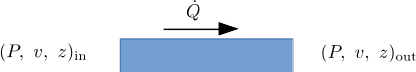
\includegraphics{hyd1.png}
\caption{Simple pipe flow}
\label{fig:hyd1}
\end{marginfigure}

\index{Bernoulli equation}
\begin{equation}
\left(\frac{P}{\gamma} + \frac{v^2}{2g}+z\right)_{\text{out}} = \left(\frac{P}{\gamma} + \frac{v^2}{2g}+z \right)_{\text{in}} + h_s - h_L
\end{equation}
where $P$ is fluid static pressure, $\gamma$ is the specific weight, $v$ is fluid velocity, $g$ is the gravitational acceleration, $z$ is fluid elevation\sidenote[][-0.5cm]{Elevation relative to an arbitrary reference.}, $h_s$ is specific shaft work, and $h_L$ is fluid head losses.\sidenote{Both $h_s$ and $h_L$ need to be specified in units of \emph{length} to be used in this equation.}

\subsection{Head Loss}
The head loss $(h_L)$ is a function of:
\begin{enumerate}
\item fluid properties---density and viscosity
\item fluid flow rate; and
\item piping system properties
\begin{enumerate}
\item pipe diameter
\item pipe material surface roughness; and
\item features of the piping system like bends, turns, elbows, flow-obstructions, etc...
\end{enumerate}
\end{enumerate}
and will be expressed as shown in Equation \ref{eq:head_loss}

\begin{equation}
h_{L} = \left(\underbrace{\frac{fL}{D}}_{\text{Major/friction}} + \underbrace{\sum k_L}_{\text{Minor/form}} \right)\frac{v^2}{2g}
\label{eq:head_loss}
\end{equation}
where $f$ is the Darcy friction factor, $L$ is the length of the piping segment between input/output, $D$ is the pipe diameter, and $k_{L}$ are coefficients characterizing minor head losses.

\index{Reynolds number}
\index{relative roughness}
\index{head loss, major}
\subsection{Major Head Losses}
In order to calculate major head losses, one needs to get a value for the Darcy friction factor $f$.  The friction factor is characterized by two dimensionless numbers: the Reynolds number\marginnote[-1.5cm]{\textbf{Reynolds number} is given by: $\text{Re} = \frac{\rho v L}{\mu}$ where $\rho$ is the fluid density, $v$ is the average fluid velocity, $L$ is a characteristic length which, for pipe-flow problems is the pipe diameter, and $\mu$ is the fluid viscosity.} and the relative roughness.\marginnote[0.25cm]{\textbf{Relative roughness} is the feature size on the surface of the pipe $(\epsilon)$ divided by the diameter of the pipe $D$}  Over a wide range of Reynolds numbers and relative roughness values the friction factor has been quantified and is traditionally displayed in graphical format in the Moody diagram as in Figure \ref{fig:moody}.

\index{Moody Diagram}
\begin{figure}
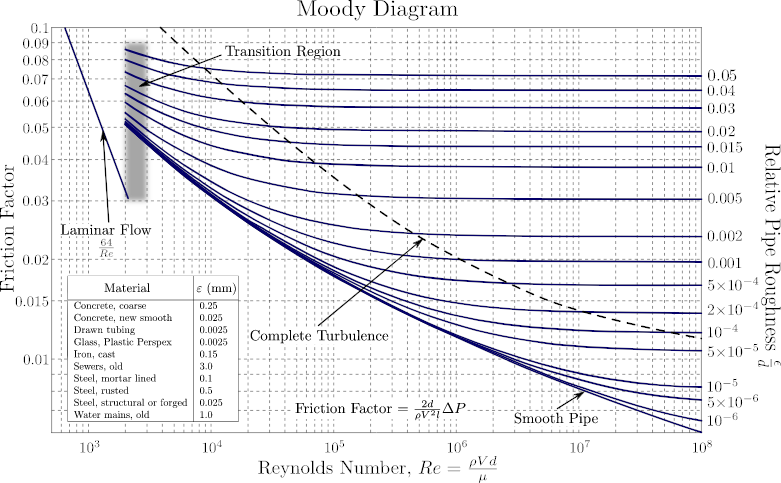
\includegraphics{moody.png}
\caption[][0cm]{The Moody Diagram for Darcy friction factor.}
\label{fig:moody}
\end{figure}

\newthought{This representation} is excellent for developing intuition on how the friction factor depends on Reynolds number and relative roughness.  In the laminar flow regime---$\ 0 \le \text{Re} \le 2000\ $---friction factor is independent of the roughness and inversely proportional to Reynolds number:
$$f = \frac{64}{\text{Re}}$$
At high Reynolds number---In the region to the right of the ``Complete Turbulence'' dashed line in Figure \ref{fig:moody}---friction factor is independent of Reynolds number and only a function of relative roughness.  Between these two regions is an area where friction factor is significantly impacted by both Reynolds number and relative roughness.

\newthought{However important} such intuition may be, computationally it may be inconvenient to \emph{require} the analyst to manually read the diagram to obtain friction factor.  An alternative approach is to use the Colebrook Equation provided in Equation \ref{eq:colebrook}.
\index{Colebrook equation}
\begin{equation}
\frac{1}{\sqrt{f}} = -2.0\log{\left(\frac{\sfrac{\epsilon}{D}}{3.7} + \frac{2.51}{\text{Re}\sqrt{f}}\right)}
\label{eq:colebrook}
\end{equation}
This equation is easily incorporated into MATLAB or Python scripts that have built-in root-finding tools allowing for parametric searches or iterative-algorithms that may be necessary for solving some hydraulic analysis problems.

\subsection{Minor Head Losses}
\newthought{Minor head losses} account for energy losses that occur when a viscous fluid flows around corners, through pipe contractions or expansions, through open or partially open valves, or any other piping feature that disrupts flow. Values for minor loss coefficients have been tabulated for many common piping system arrangements and, for the typical student of ER468, has already been studied in EM324 Fluid Dynamics.  

In ER468 we seek to extend that training to include nuclear-specific design features that contribute to minor head losses.  These include minor losses due to:
\begin{itemize}
\item flow past nuclear fuel rod bundles in either rectangular or hexagonal arrangements, including those fitted with mixing vanes and structural spacer grids; and
\item flow through heat exchangers fitted with enhanced surface features intended for improvement of convective heat transfer 
\end{itemize}

\subsection{Fluid Flow Problem Types}

In EM324 we discussed three hydraulic problem types:
\begin{itemize}
\item Type I---volumetric flow rate and pipe geometry given: find head loss;
\item Type II---pipe geometry and head loss given: find volumetric flow rate; and
\item Type III---head loss and volumetric flow rate given: find pipe geometry (e.g. diameter)
\end{itemize}

Most of the problems that we will pose in this class will fall into the Type I category and this category is in many ways the easiest.  Due to the non-linear nature of Equation \ref{eq:colebrook} problems of Type II or Type III generally require an iterative solution approach.  Nonetheless, problems of these types are definitely relevant for the engineering analysis of a nuclear reactor.  A thermal analysis of the core may dictate a given mass or volumetric flow rate; other limitations may impose some constraint on allowable head loss and your goal is to find an acceptable geometry.  A well-prepared nuclear engineer should be able to meet any of these challenges.

\begin{margintable}
\begin{tabular}{|c|c|}
\hline
Parameter & Value \\
\hline
Density & 42.282 $\text{lb}_{\text{m}}/\text{ft}^3$ \\
\hline
Viscosity & $1.67 \times 10^{-6} \text{lb}_{\text{m}}/\text{ft-s}$ \\
\hline
Mass flow rate & 16,744 $\text{lb}_{\text{m}}$/s \\
\hline
\end{tabular}
\caption{Fluid properties for example problem}
\label{tab:ex_props15}
\end{margintable}

\begin{example}
\textbf{Example:} The hot leg of an AP1000 reactor is 16 ft long and has an inside diameter of 31 inches.  The piping material has a relative roughness of 0.001.  The fluid properties of water in the hot leg are constant and given in Table \ref{tab:ex_props15}.  Assume that a) the hot leg piping is of constant diameter; b) that minor losses are negligible, and c) that the hot leg piping is on roughly the same elevation from the reactor vessel outlet to the steam generator inlet. \textbf{Find:} the pressure drop (psid) as coolant flows through the hot leg.
\end{example}

\textbf{Solution:} 
From the Bernoulli equation under given assumptions:
$$\left(\frac{P}{\gamma} + \cancel{\frac{v^2}{2g}}+\cancel{z}\right)_{\text{out}} = \left(\frac{P}{\gamma} + \cancel{\frac{v^2}{2g}}+\cancel{z} \right)_{\text{in}} + \cancelto{0}{h_s} - h_L   $$
where the kinetic and potential energy terms are eliminated since they do not change over the length of the hot leg piping.  This leaves:
$$ \frac{P_{\text{in}}-P_{\text{out}}}{\gamma} = h_L = \frac{fL}{D}\frac{v^2}{2g}$$
The velocity is obtained from the continuity equation: $\dot{m}=\rho v A$ where $A$ is the cross-sectional area of the piping.  Thus:
$$v = \frac{\dot{m}}{\rho A} = 75.6 \text{ft/s}$$
With the velocity, Reynolds number can be found:
$$\text{Re} = \frac{\rho v D}{\mu} = 4.9\times 10^{9}$$
which is sadly off the scale of Figure \ref{fig:moody} but definitely falls into the ``Complete Turbulence'' region so the friction factor can be obtained from the relative roughness alone.  Since $\sfrac{\epsilon}{D} = 0.001$, reading the Moody chart gives us a Darcy Friction factor: $f \approx 0.02$.  

Applying these calculated values with appropriate conversion factors\marginnote{\textbf{Note: } $\gamma$ is the specific weight, but the density was given.  In the USCS unit system, $\gamma = \rho \frac{g_c}{g}$ where $g_c = 32.2 \frac{\text{lb}_{\text{f}}}{\text{lb}_{\text{m}}}\frac{\text{ft}}{\text{s}^2}  $ and $g=32.2 \frac{\text{ft}}{s^2}$ thus $\gamma = 42.282 \frac{\text{lb}_f}{\text{ft}^3}$.} gives us our result:
$$\Delta P = 3.2 \text{ psid}$$.




